\documentclass[9pt,twoside,lineno]{pnas-new}
% Use the lineno option to display guide line numbers if required.

\templatetype{pnassupportinginfo}
% \readytosubmit %% Uncomment this line before submitting, so that the instruction page is removed.

\usepackage{tabstackengine}
\setstackEOL{\cr}

\title{Your Main Manuscript Title}
\author{Author1, Author2 and Author3 (Complete author list)}
\correspondingauthor{Corresponding Author Name.\\E-mail: author.two@email.com}

\begin{document}

%% Comment/remove this line before generating final copy for submission
\instructionspage  

\maketitle

%% Adds the main heading for the SI text. Comment out this line if you do not have any supporting information text.
\SItext


\section*{Deriving motion equations}

\begin{figure}[tbhp]
\centering
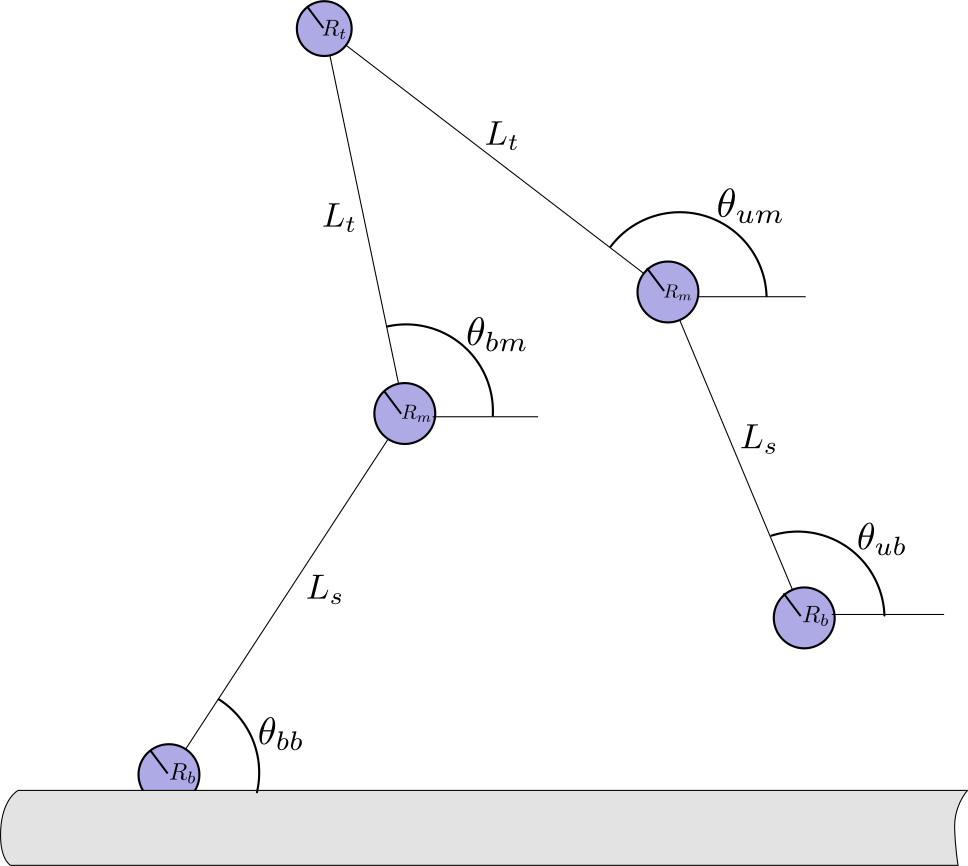
\includegraphics[width=0.49\linewidth]{figures/onebound-cartoon.pdf}
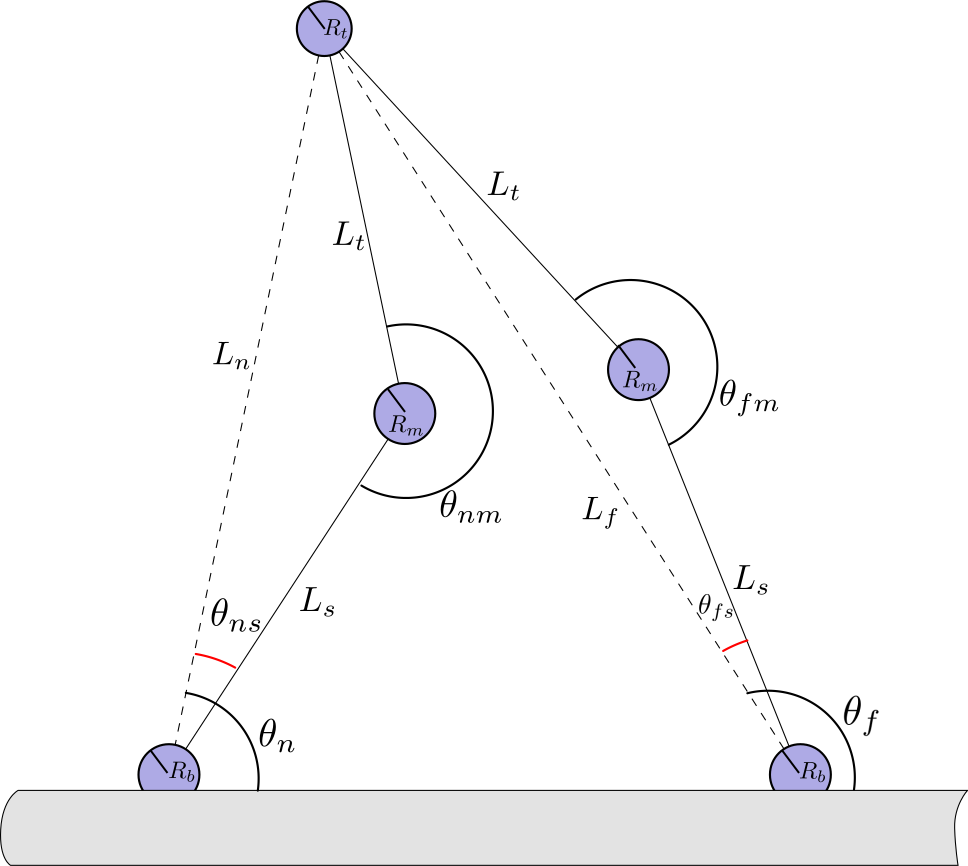
\includegraphics[width=0.49\linewidth]{figures/bothbound-cartoon.pdf}
\caption{}
\label{fig:supp-model}
\end{figure}


\subsection*{Onebound case}
The following equations allow recursive calculation of the positions of each domain in Cartesian coordinates:

\noindent\begin{minipage}{0.49\linewidth}
\begin{align}
  X_{bm} &= X_{bb}+L_{s}\cos(\theta_{bb}) \\
  X_{t}  &= X_{bm}+L_{t}\cos(\theta_{bm}) \\
  X_{fm} &= X_{t} - L_{t}\cos(\theta_{fm}) \\
  X_{fb} &= X_{fm} - L_{s}\cos(\theta_{fb})
\end{align}
\end{minipage}
\begin{minipage}{0.49\linewidth}
\begin{align}
  Y_{bb} &= 0 \\
  Y_{bm} &= Y_{bb}+L_{s}\sin(\theta_{bb}) \\
  Y_{t}  &= Y_{bm}+L_{t}\sin(\theta_{bm}) \\
  Y_{fm} &= Y_{t} - L_{t}\sin(\theta_{fm}) \\
  Y_{fb} &= Y_{fm} - L_{s}\sin(\theta_{fb})
\end{align}
\end{minipage}
\vspace{.5cm}

$L_s$ and $L_t$ correspond to lengths of each interdomain rod, and the $t$ subscripts refer to tail domain coordinates.\\

The goal is to express angular velocities $\dot{\theta}_{bb}, \dot{\theta}_{bb}, \dot{\theta}_{bb}$ and $\dot{\theta}_{bb}$ in terms of known quantities. To begin, the Cartesian velocities of each domain can be calculated from the above position equations in a similar recursive manner. A subset of the equations are shown here:

\noindent\begin{minipage}{0.49\linewidth}
\begin{align}
  \dot{X}_{bb} &= 0 \\
  \dot{X}_{bm} &= \dot{X}_{bb} - L_{s}\sin(\theta_{bb})\dot{\theta}_{bb} \label{cartesian-bmx}\\
  \dot{X}_{t } &= \dot{X}_{bm} - L_{t}\sin(\theta_{bm})\dot{\theta}_{bm}
  %% \dot{X}_{fm} &= \dot{X}_{t } + L_{t}\sin(\theta_{fm})\dot{\theta}_{fm} \\
  %% \dot{X}_{fb} &= \dot{X}_{fm} + L_{s}\sin(\theta_{fb})\dot{\theta}_{fb}
\end{align}
\end{minipage}
\begin{minipage}{0.49\linewidth}
\begin{align}                                                                          
  \dot{Y}_{bb} &= 0 \\                                                        
  \dot{Y}_{bm} &= \dot{Y}_{bb} + L_{s}\cos(\theta_{bb})\dot{\theta}_{bb} \\
  \dot{Y}_{t}  &= \dot{Y}_{bm} + L_{t}\cos(\theta_{bm})\dot{\theta}_{bm}
  %% \dot{Y}_{fm} &= \dot{Y}_{t } - L_{t}\cos(\theta_{fm})\dot{\theta}_{fm} \\
  %% \dot{Y}_{fb} &= \dot{Y}_{fm} - L_{s}\cos(\theta_{fb})\dot{\theta}_{fb}
\end{align}
\end{minipage}
\vspace{.5cm}

Another way to express these Cartesian velocities is using the Brownian dynamics equation $\dot{X} = \frac1\gamma F_{net} + R$:

\begin{align}  
  \dot{X}_{bm} &= \frac{1}{\gamma_m} \Big(F_{xml} + - \lambda_{bs}(X_{bm} - X_{bb}) + \lambda_{bt}(X_{t } - X_{bm}) \Big) + R_{xml} \label{brownian-bmx}\\
  \dot{X}_{t } &= \frac{1}{\gamma_t} \Big(F_{xt } + - \lambda_{bt}(X_{t } - X_{bm}) + \lambda_{ft}(X_{fm} - X_{t }) \Big) + R_{xt }
  %% \dot{X}_{fm} &= \frac{1}{\gamma_m} \Big(F_{xmr} + - \lambda_{ft}(X_{fm} - X_{t }) + \lambda_{fs}(X_{fb} - X_{fm}) \Big) + R_{xmr} \\
  %% \dot{X}_{fb} &= \frac{1}{\gamma_b} \Big(F_{xbr} + - \lambda_{fs}(X_{fb} - X_{fm}) \Big) + R_{xbr}
\end{align}
%
where $\gamma_n$ is a drag coefficient for the binding, motor or tail domain with units of mass per second. $F_{xn}$ is the x component of external force on each domain $n$ due to various factors. $\lambda_{12}\left(X_1 - X_2\right)$ is the x component of internal force on domain $2$ due to domain $1$, where $\lambda$ is a tension coefficient with units of mass per second squared, also known as a Lagrange multiplier. $R_{xn}$ is the Brownian coefficient representing motion due to solvent collision, with units of velocity.\\

These two sets of equations, Cartesian and Brownian, can be equated to get more interesting equations. For example, Eq (\ref{cartesian-bmx}) and Eq (\ref{brownian-bmx}) can be equated. This equating, combined with expanding the recursive velocity definitions leads to new equations, some of which are shown here:

\begin{align}
  &-L_s\sin(\theta_{bb})\dot{\theta}_{bb} = \frac{1}{\gamma_m}F_{xml} + -\frac{1}{\gamma_m}\lambda_{bs}(X_{bm} - X_{bb}) + \frac{1}{\gamma_m}\lambda_{bt}(X_{t } - X_{bm}) + R_{bmx} \label{ob_system_first}\\
  &-L_s\sin(\theta_{bb})\dot{\theta}_{bb} - L_t\sin(\theta_{bm})\dot{\theta}_{bm} = \frac{1}{\gamma_t}F_{xt } + -\frac{1}{\gamma_t}\lambda_{bt}(X_{t } - X_{bm}) + \frac{1}{\gamma_t}\lambda_{ft}(X_{um} - X_{t }) + R_{tx}\label{ob_system_second}
\end{align}
%
A total of eight coupled differential equations are formed from this procedure. These eight equations form a system of equations with eight unknowns: $\dot{\theta}_{bb}, \dot{\theta}_{bb}, \dot{\theta}_{bb}$ and $\dot{\theta}_{bb}$, and the four tension coefficients $\lambda_{bs}, \lambda_{bt}, \lambda_{um}$ and $\lambda_{ub}$. This system is more compactly represented as:

\setstacktabbedgap{4pt}
{\tiny
  \[
  \hspace{-1.0cm}
  \resizebox{0.85\linewidth}{!}{%
    $\parenMatrixstack{
      L_s\sin\theta_{bb} & 0 & 0 & 0 & -\gamma_m (X_{bm} - X_{bb}) & \gamma_m (X_{t } - X_{bm}) & 0 & 0 \cr
      L_s\sin(\theta_{bb}) & L_t\sin(\theta_{bm}) & 0 & 0 & 0 & -\gamma_t (X_{t } - X_{bm}) & \gamma_t (X_{um} - X_{t }) & 0 \cr
      L_s\sin(\theta_{bb}) & L_t\sin(\theta_{bm}) & -L_t\sin(\theta_{um}) & 0 & 0 & 0 & -\gamma_m (X_{um} - X_{t }) & \gamma_m (X_{ub} - X_{um}) \cr
      L_s\sin(\theta_{bb}) & L_t\sin(\theta_{bm}) & -L_t\sin(\theta_{um}) & -L_s\sin(\theta_{ub}) & 0 & 0 & 0 & -\gamma_b (X_{ub} - X_{um}) \cr
      -L_s\cos(\theta_{bb}) & 0 & 0 & 0 & -\gamma_m (Y_{bm} - Y_{bb}) & \gamma_m (Y_{t } - Y_{bm}) & 0 & 0 \cr
      -L_s\cos(\theta_{bb}) & -L_t\cos(\theta_{bm}) & 0 & 0 & 0 & -\gamma_t (Y_{t } - Y_{bm}) & \gamma_t (Y_{um} - Y_{t }) & 0 \cr
      -L_s\cos(\theta_{bb}) & -L_t\cos(\theta_{bm}) & L_t\cos(\theta_{um}) & 0 & 0 & 0 & -\gamma_m (Y_{um} - Y_{t }) & \gamma_m (Y_{ub} - Y_{um}) \cr
      -L_s\cos(\theta_{bb}) & -L_t\cos(\theta_{bm}) & L_t\cos(\theta_{um}) & L_s\cos(\theta_{ub}) & 0 & 0 & 0 & -\gamma_b (Y_{ub} - Y_{um})
      }$%
    }
  \begin{pmatrix}
    \dot{\theta}_{bb}\\
    \dot{\theta}_{bm}\\
    \dot{\theta}_{um}\\
    \dot{\theta}_{ub}\\
    \lambda_{bs}\\
    \lambda_{bt}\\
    \lambda_{ut}\\
    \lambda_{us}\\
  \end{pmatrix}
  =
  \begin{pmatrix}
    -F_{bmx} + \gamma_m R_{bmx}\\
    -F_{tx} + \gamma_t R_{tx}\\
    -F_{umx} + \gamma_m R_{umx}\\
    -F_{ubx} + \gamma_b R_{ubx}\\
    -F_{bmy} + \gamma_m R_{bmy}\\
    -F_{ty} + \gamma_t R_{ty}\\
    -F_{umy} + \gamma_m R_{umy}\\
    -F_{uby} + \gamma_b R_{uby}\\
  \end{pmatrix}
  \]
}

This matrix is then solved using the Mathematica computer algebra system, resulting in a set of motion equations which describe the model's trajectory over time, e.g. $\dot{\theta_{bm}}(\theta_{bb}, \theta_{bm}, \theta_{um}, \theta_{ub})$. These motion equations are further described in Appendix (\ref{sec:AppendixOneboundEquations}).\\

\subsection*{Bothbound case}
The first step in calculating angular velocities is to define intermediate variables $L_n$ and $L_f$ using the law of cosines:

\begin{align}
  L_n &= \sqrt{L_s^2 + L_t^2 - 2L_sL_t\cos{\theta_{nm}}} \\
  L_f &= \sqrt{L_s^2 + L_t^2 - 2L_sL_t\cos{\theta_{fm}}}
\end{align}

These new artificial stalks are not physically relevant, but allow the definition of new angles $\theta_n, \theta_{ns}, \theta_{f}$ and $\theta_{fs}$, which are useful for calculating the position of the motor domain. The treatment of the near and far versions of these angles is very similar, so only the near angles will be dealt with here. The angles themselves are never dealt with, only their sines and cosines:

\begin{align}
  \cos\theta_n &= \frac{L^2 + L_n^2 - L_f^2}{2L L_n} \\
  \sin\theta_{n} &= \sqrt{1 - \cos^2\theta_{n}} \\
  \cos\theta_{ns} &= \frac{L_s^2 + L_n^2 - L_t^2}{2L_s L_n} \\
  \sin\theta_{ns} &=
  \begin{cases}
    +\sqrt{1 - \cos^2\theta_{ns}} & \theta_{nm} < \pi \\
    -\sqrt{1 - \cos^2\theta_{ns}} & \theta_{nm} > \pi
  \end{cases}
\end{align}

These values are arrived at through the Law of Cosines and a trigonometric identity. The sign of $\sin\left(\theta_n\right)$ is restricted to positive values due to the angle's $[0,\pi]$ domain. $\theta_{ns}$'s domain is $[-\pi,\pi]$, meaning its sign is not restricted. The partial derivatives of these values are used in future calculations, and some are shown here:

\begin{align}
  \frac{\partial \cos\theta_n}{\partial L_n} &= \frac{1}{L} - \frac{L^2 + L_n^2 - L_f^2}{2L L_n^2}\\
  \frac{\partial \cos\theta_n}{\partial L_f} &= -\frac{L_f}{LL_n}\\
  \frac{\partial \sin\theta_n}{\partial L_n} &= \frac{-\cos\theta_n}{\sqrt{1-\cos^2\theta_n}}
  \left(\frac{1}{L} - \frac{L^2 + L_n^2 - L_f^2}{2L L_n^2}\right)
  %% \frac{\partial \sin\theta_n}{\partial L_f} &= \frac{-\cos\theta_n}{\sqrt{1-\cos^2\theta_n}}
  %% \left(\frac{-L_f}{LLn}\right)\\
  %% \frac{\partial \cos\theta_{ns}}{\partial L_n} &= \frac{1}{L_s}
  %% - \frac{L_s^2 + L_n^2 - L_t^2}{2L_sL_n^2}\\
  %% \frac{\partial \cos\theta_{ns}}{\partial L_f} &= 0\\
  %% \frac{\partial \sin\theta_{ns}}{\partial L_n} &=
  %% \begin{cases}
  %%   \frac{-\cos\theta_{ns}}{\sqrt{1-\cos^2\theta_{ns}}}
  %%   \left(\frac{1}{L_s} - \frac{L_s^2+L_n^2-L_t^2}{2LL_n^2}\right) & \theta_{nm} < \pi \\
  %%   \frac{\cos\theta_{ns}}{\sqrt{1-\cos^2\theta_{ns}}}
  %%   \left(\frac{1}{L_s} - \frac{L_s^2+L_n^2-L_t^2}{2LL_n^2}\right) & \theta_{nm} > \pi
  %% \end{cases}\\
  %% \frac{\partial \sin\theta_{ns}}{\partial L_f} &= 0
\end{align}
%
The position of the motor and tail domains is calculated as follows, using the angle addition trigonometric identity:

\begin{align}
  X_{nm} &= L_s\left(
  \cos\theta_n\cos\theta_{ns} - \sin\theta_n\sin\theta_{ns}
  \right)
  \\
  Y_{nm} &= L_s\left(
  \cos\theta_n\sin\theta_{ns} + \sin\theta_n\cos\theta_{ns}
  \right)
  \\
  X_{t} &= L_n\cos\theta_n\\
  Y_{t} &= L_n\sin\theta_n
\end{align}

The partial derivatives of these values are used later. A selection are shown here:

\begin{align}
  \frac{dX_{nm}}{dL_n} &= L_s\Big(\cos\theta_n\frac{d\cos\theta_{ns}}{dL_n} + \cos\theta_{ns}\frac{d\cos\theta_{n}}{dL_n} - \sin\theta_n\frac{d\sin\theta_{ns}}{dL_n} - \sin\theta_{ns}\frac{d\sin\theta_{n}}{dL_n}\Big)\\
  \frac{dY_{nm}}{dL_n} &= L_s\Big(\cos\theta_n\frac{d\sin\theta_{ns}}{dL_n} + \sin\theta_{ns}\frac{d\cos\theta_{n}}{dL_n} + \sin\theta_n\frac{d\cos\theta_{ns}}{dL_n} + \cos\theta_{ns}\frac{d\sin\theta_{n}}{dL_n} \Big)\\
  \frac{dX_{nm}}{dL_f} &= L_s\Big(\cos\theta_n\frac{d\cos\theta_{ns}}{dL_f} + \cos\theta_{ns}\frac{d\cos\theta_{n}}{dL_f} - \sin\theta_n\frac{d\sin\theta_{ns}}{dL_f} - \sin\theta_{ns}\frac{d\sin\theta_{n}}{dL_f} \Big)
  %% \frac{dY_{nm}}{dL_f} &= L_s\Big(\cos\theta_n\frac{d\sin\theta_{ns}}{dL_f} + \sin\theta_{ns}\frac{d\cos\theta_{n}}{dL_f} + \sin\theta_n\frac{d\cos\theta_{ns}}{dL_f} + \cos\theta_{ns}\frac{d\sin\theta_{n}}{dL_f}\Big)\\
  %% \frac{dX_{t}}{dL_n} &= \cos\theta_n + L_n\frac{\partial \cos\theta_n}{\partial L_n} = \frac{L_n}{L}\\
  %% \frac{dY_{t}}{dL_n} &= \sin\theta_n + L_n\frac{\partial \sin\theta_n}{\partial L_n}\\
  %% \frac{dX_{t}}{dL_f} &= L_n\frac{\partial \cos\theta_n}{\partial L_f} = -\frac{L_f}{L}\\
  %% \frac{dY_{t}}{dL_f} &= L_n\frac{\partial \sin\theta_n}{\partial L_f}\\
\end{align}
%
These partial derivatives are then used in a system of equations very similar to that in Equations (\ref{ob_system_first}-\ref{ob_system_second}), combining Brownian and coordinate system definitions of domain velocities:

\begin{align}
  \dot{X}_{nm} &= \frac{1}{\gamma} \Big(F_{xml} - \lambda_{ns}(X_{bm} - X_{bb})
  + \lambda_{nt}(X_{t } - X_{bm}) \Big) + R_{xml}
  &=& \frac{\partial X_{nm}}{\partial L_n}\dot{L}_n + \frac{\partial X_{nm}}{\partial L_f}\dot{L}_f\\
  \dot{X}_{t } &= \frac{1}{\gamma} \Big(F_{xt } - \lambda_{nt}(X_{t } - X_{bm})
  + \lambda_{ft}(X_{fm} - X_{t }) \Big) + R_{xt }
  &=& \frac{\partial X_{t}}{\partial L_n}\dot{L}_n + \frac{\partial X_{t}}{\partial L_f}\dot{L}_f\\
  \dot{X}_{fm} &= \frac{1}{\gamma} \Big(F_{xmr} - \lambda_{ft}(X_{fm} - X_{t })
  + \lambda_{fs}(X_{fb} - X_{fm}) \Big) + R_{xmr}
  &=& \frac{\partial X_{fm}}{\partial L_n}\dot{L}_n + \frac{\partial X_{fm}}{\partial L_f}\dot{L}_f
\end{align}

\begin{align}
  \dot{Y}_{nm} &= \hspace{1cm} \frac{1}{\gamma} \Big(F_{yml} - \lambda_{ns}(Y_{bm} - Y_{bb})
  + \lambda_{nt}(Y_{t } - Y_{bm}) \Big) + R_{yml}
  &= \frac{\partial Y_{nm}}{\partial L_n}\dot{L}_n + \frac{\partial Y_{nm}}{\partial L_f}\dot{L}_f\\
  \dot{Y}_{t}  &= \hspace{1cm} \frac{1}{\gamma} \Big(F_{yt } - \lambda_{nt}(Y_{t } - Y_{bm})
  + \lambda_{ft}(Y_{fm} - Y_{t }) \Big) + R_{yt }
  &= \frac{\partial Y_{t}}{\partial L_n}\dot{L}_n + \frac{\partial Y_{t}}{\partial L_f}\dot{L}_f\\
  \dot{Y}_{fm} &= \hspace{1cm} \frac{1}{\gamma} \Big(F_{ymr} - \lambda_{ft}(Y_{fm} - Y_{t })
  + \lambda_{fs}(Y_{fb} - Y_{fm}) \Big) + R_{ymr}
  &= \frac{\partial Y_{fm}}{\partial L_n}\dot{L}_n + \frac{\partial Y_{fm}}{\partial L_f}\dot{L}_f
\end{align}
%
The matrix version of this system looks like:

\[
\begin{pmatrix}
  -\frac{X_{nm}}{Ln} & -\frac{X_{nm}}{Lf}
  & -\frac{X_{nm}-X_{nb}}{\gamma} & \frac{X_{t}-X_{nm}}{\gamma} & 0 & 0\\
  -\frac{X_{t}}{Ln} & -\frac{X_{t}}{Lf}
  & 0 & -\frac{X_{t}-X_{nm}}{\gamma} & \frac{X_{fm}-X_{t}}{\gamma} & 0\\
  -\frac{X_{fm}}{Ln} & -\frac{X_{fm}}{Lf}
  & 0 & 0 & -\frac{X_{fm}-X_{t}}{\gamma} & \frac{X_{fb}-X_{fm}}{\gamma}\\
  -\frac{Y_{nm}}{Ln} & -\frac{Y_{nm}}{Lf}
  & -\frac{Y_{nm}-Y_{nb}}{\gamma} & \frac{Y_{t}-Y_{nm}}{\gamma} & 0 & 0\\
  -\frac{Y_{t}}{Ln} & -\frac{Y_{t}}{Lf}
  & 0 & -\frac{Y_{t}-Y_{nm}}{\gamma} & \frac{Y_{fm}-Y_{t}}{\gamma} & 0\\
  -\frac{Y_{fm}}{Ln} & -\frac{Y_{fm}}{Lf}
  & 0 & 0 & -\frac{Y_{fm}-Y_{t}}{\gamma} & \frac{Y_{fb}-Y_{fm}}{\gamma}\\
\end{pmatrix}
\begin{pmatrix}
  \dot{L}_n\\
  \dot{L}_f\\
  \lambda_{ns}\\
  \lambda_{nt}\\
  \lambda_{ft}\\
  \lambda_{fs}\\
\end{pmatrix}
=
\begin{pmatrix}
  -\frac{1}{\gamma}F_{nmx} - R_{nmx}\\
  -\frac{1}{\gamma}F_{tx}  - R_{tx}\\
  -\frac{1}{\gamma}F_{fmx} - R_{fmx}\\
  -\frac{1}{\gamma}F_{nmy} - R_{nmy}\\
  -\frac{1}{\gamma}F_{ty}  - R_{ty}\\
  -\frac{1}{\gamma}F_{fmy} - R_{fmy}\\
\end{pmatrix}
\]
%
This system of equations is then solved and used to calculate $\dot{L}_n$ and $\dot{L}_f$, as shown in Appendix (\ref{sec:AppendixBothboundEquations}). These intermediate velocities can then be used to calculate $\dot{\theta_{nm}}$ and $\dot{\theta_{fm}}$.\\

\section*{Simulation special cases}
Model time evolution led to certain special cases which required attention:\\

\textbf{Domain below microtubule:} When a domain's velocity would result in the domain's y value becoming negative, the velocity was rejected and a new one calculated. The stochastic nature of $R$ guarentees that eventually a velocity would be selected which doesn't lead to a negative y value.\\

\textbf{$\theta_{nm}$ or $\theta_{fm}$ approach $\pi/2$:} Bothbound velocity calculations would yield NaNs when motor angles approached $\pi/2$. To prevent this, random perturbations of $1e-5$ were added to each motor angle when it was sufficiently close to $\pi/2$.

\section*{Fitting spring constants}
How we fit spring constants; maybe plot the 3d correlation-color scatter plot for 3 springs

\begin{figure}[tbhp]
\centering
%% 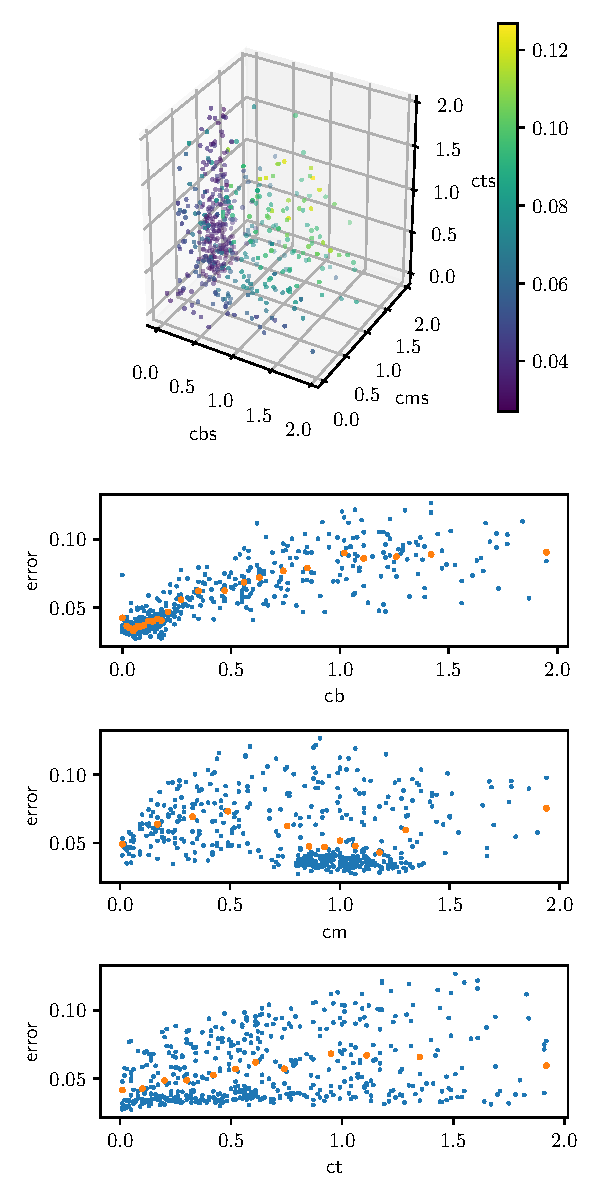
\includegraphics[width=0.7\linewidth]{../../plots/randomsearchplot.pdf}
FIXME WHERE DOES randomsearchplot.pdf come from?
\caption{\textbf{Fitting spring constants through homology to experimental stepping data.} \textit{A.} 3D scatter plot of simulations color-coded by the sum-of-squares error between the model and experimental stepping histograms. \textit{B-D:} Scatter plots of spring constants and error; orange dots indicate averages over nearest 25 points.}
\label{fig:supp-model-fit}
\end{figure}

%% \section*{Foot order statistics}

%% \begin{figure}[tbhp]
%% \centering
%% \includegraphics[width=0.7\linewidth]{../../plots/paper_foot_order_statistics.pdf}
%% \caption{\textbf{Foot order statistics}}
%% \label{fig:supp-foot-order}
%% \end{figure}


%%% Each figure should be on its own page
%% \begin{figure}
%% \centering
%% \includegraphics[width=\textwidth]{example-image}
%% \caption{First figure}
%% \end{figure}

%% \begin{figure}
%% \centering
%% \includegraphics[width=\textwidth]{frog}
%% \caption{Second figure}
%% \end{figure}

%% \begin{table}\centering
%% \caption{This is a table}

%% \begin{tabular}{lrrr}
%% Species & CBS & CV & G3 \\
%% \midrule
%% 1. Acetaldehyde & 0.0 & 0.0 & 0.0 \\
%% 2. Vinyl alcohol & 9.1 & 9.6 & 13.5 \\
%% 3. Hydroxyethylidene & 50.8 & 51.2 & 54.0\\
%% \bottomrule
%% \end{tabular}
%% \end{table}

%%% Add this line AFTER all your figures and tables
\FloatBarrier

%% \movie{Type caption for the movie here.}

%% \movie{Type caption for the other movie here. Adding longer text to show what happens, to decide on alignment and/or indentations.}

%% \movie{A third movie, just for kicks.}

%% \dataset{dataset_one.txt}{Type or paste caption here.}

%% \dataset{dataset_two.txt}{Type or paste caption here. Adding longer text to show what happens, to decide on alignment and/or indentations for multi-line or paragraph captions.}

%% \bibliography{pnas-sample}

\end{document}
              
            
